\documentclass[]{report}


\usepackage[autostyle]{csquotes} 
\usepackage{parskip}
\usepackage{graphicx}
\usepackage{placeins}
\usepackage{wrapfig}
\usepackage{epigraph}
\usepackage[T1]{fontenc}
\usepackage{titlesec, blindtext, color}
\definecolor{gray75}{gray}{0.75}
\newcommand{\hsp}{\hspace{20pt}}
\titleformat{\chapter}[hang]{\Huge\bfseries}{\thechapter\hsp\textcolor{gray75}{|}\hsp}{0pt}{\Huge\bfseries}
\makeatletter
\newif\if@right
\def\shadequote{\@righttrue\shadequote@i}
\def\shadequote@i{\begin{snugshade}\begin{quote}\openquote}
\def\endshadequote{%
  \if@right\hfill\fi\closequote\end{quote}\end{snugshade}}
\@namedef{shadequote*}{\@rightfalse\shadequote@i}
\@namedef{endshadequote*}{\endshadequote}
\makeatother


\newcommand\todo[1]{\textcolor{red}{TODO: }#1\PackageWarning{TODO:}{TODO tag!!}}



\usepackage{listings}
\usepackage{color}
\usepackage{courier}

\definecolor{dkgreen}{rgb}{0,0.6,0}
\definecolor{gray}{rgb}{0.5,0.5,0.5}
\definecolor{mauve}{rgb}{0.58,0,0.82}

\lstset{frame=tb,
  language=[Sharp]C,
  aboveskip=3mm,
  belowskip=3mm,
  showstringspaces=false,
  columns=flexible,
  basicstyle={\small\ttfamily},
  numbers=none,
  numberstyle=\tiny\color{gray},
  keywordstyle=\color{blue},
  commentstyle=\color{dkgreen},
  stringstyle=\color{mauve},
  breaklines=true,
  breakatwhitespace=true
  tabsize=3
}




\begin{document}

\graphicspath{{img/}{../img/}}
\begin{titlepage}
\begin{center}

\vspace{2cm}

\centering
\includegraphics[width=300px]{/logo.png}

\vspace{1cm}

\rule{\linewidth}{0.6mm}

\textsc{\LARGE OCON}\\
\textsc{\large A context-awareness framework}
\vspace{0.2cm}
\rule{\linewidth}{0.4mm}

Jacob B. \textsc{Cholewa}
\\ \& \\
Mathias K. \textsc{Pedersen}

\vfill

\large \today
\end{center}


\end{titlepage}

\begin{abstract}
\end{abstract}


\chapter{Project description}
A Context-aware system is able to adapt its behavior to the surroundings it is in. In order to act upon its environment, the system will need sensor-input. Various sources of input can be used to determine the actions of the system.\\

In this project we want to mainly focus on implementing a context-awareness framework, making it easy for systems to actuate on sensor events. As a proof of concept we will explore replacing the physical SCRUM board, which is often a whiteboard and post-its, with an IT-solution which is not confined to a personal computer, but has the same presence. The digital SCRUM board will be context-aware to the extent that it can recognize different SCRUM activities, like sprint meeting or one-on-one, and automatically change its graphical interface.


\chapter{Scope of this project}

As per our Project description there are two artifacts to be made; The context awareness framework and a proof of concept implementation in form of a Context-aware Scrum board.

\paragraph{The Framework.} 
Our project description dictates that the main piece of work will be our framework, and so implementation of this framework will have the broadest scope.\\

\begin{itemize}
\item[\textbf{Goal 1 }] \textit{Our aim is to implement a framework that is adaptable and easy to use.}
\end{itemize}


\paragraph{The Scrum board.} 
For us to prove usability of the framework developed we will implement it for a context-aware Scrum board. The function of this artifact is solely to test the usefulness of the context-awareness framework.\\

\begin{itemize}
\item[\textbf{Goal 2 }] \textit{In trying to prove Goal 1, implement a stub Scrum board utilizing the framework}
\end{itemize}

It is not in our scope to implement a functional or useful Scrum board.








\chapter{Background Research}
\section{Context awareness}
To be able to make a context-aware framework, we first had to investigate what context and context-awareness is in a computer science perspective.

Context-awareness is a term associated with Ubiquitous computing. Ubiquitous computing, ubicomp, was coined in the early nineties by Mark Weiser whose vision was to make technology that could seamlessly assist in everyday tasks. Weisers research-unit at Xerox PARC developed some of the first mobile devices, and the development of ubi computing clearly reflects in todays technology boom of smart phones and tablets.

For a system to seamlessly interact with a human the system must acquire knowledge to the current situation or \textit{context}. Many of the publications on the subject describes context different, but the one description fitting best our understanding was coined by Dey and Abowd whom described context as:

\blockquote{\textit{Any information that can be used to characterize the situation of an entity. An entity is a person, place or object that is considered relevant to the interaction between a user and an application, including the user and application themselves.}} \cite{Dey and Abowd (2000)} 

When humans interact, they can interpret the ongoing situation from implicitly understanding body language, tone of voice, the surrounding environment as well as maybe having a relation to the person or knowing about past and future events. These \textit{context informations} is essential factors in effective communication. By increasing the amount of context information available to computers, human-machine interaction can be improved.\\

% Holy grail is to understand and perform human intent
\todo{We strive to understand human intent, with sensors. We might not catch it all, but that's not because it's a machine, this can happen in all kinds of interactions; culture differneces... Something on this}


Much research have been done in increasing the available amount of context-information, but also heightening the quality and correctness of the information is in focus. As the amount of context increases, the context-aware application becomes able to take actions without explicit user input. When doing so, action can be taken on wrong or typically incomplete snaps of context. 


\blockquote{\textit{Intelligibility and control are important user concerns in context-aware applications. They allow a user to understand why an application is behaving a certain way, and to change its behavior.}} \cite{Dey and Newberger (2009)}

\todo Write more about context accuracy


\section{Context aware frameworks}
% Frameworks have been developed to accomadate this
To support application developers a number of context-frameworks have been developed. When looking at the frameworks mainly two approaches were used: Blackboard and Widget-based architecture.

The blackboard approach is a centralized solution. Sensors and application are connected to the blackboard and when ever a new sensor state is available a post-it, an entry to the database, is put on the blackboard. The application can at will look through the blackboard and search for context it might find relevant. The blackboard abstracts away the sensor allowing the client to focus on only the context information. 

\begin{figure}
\centering
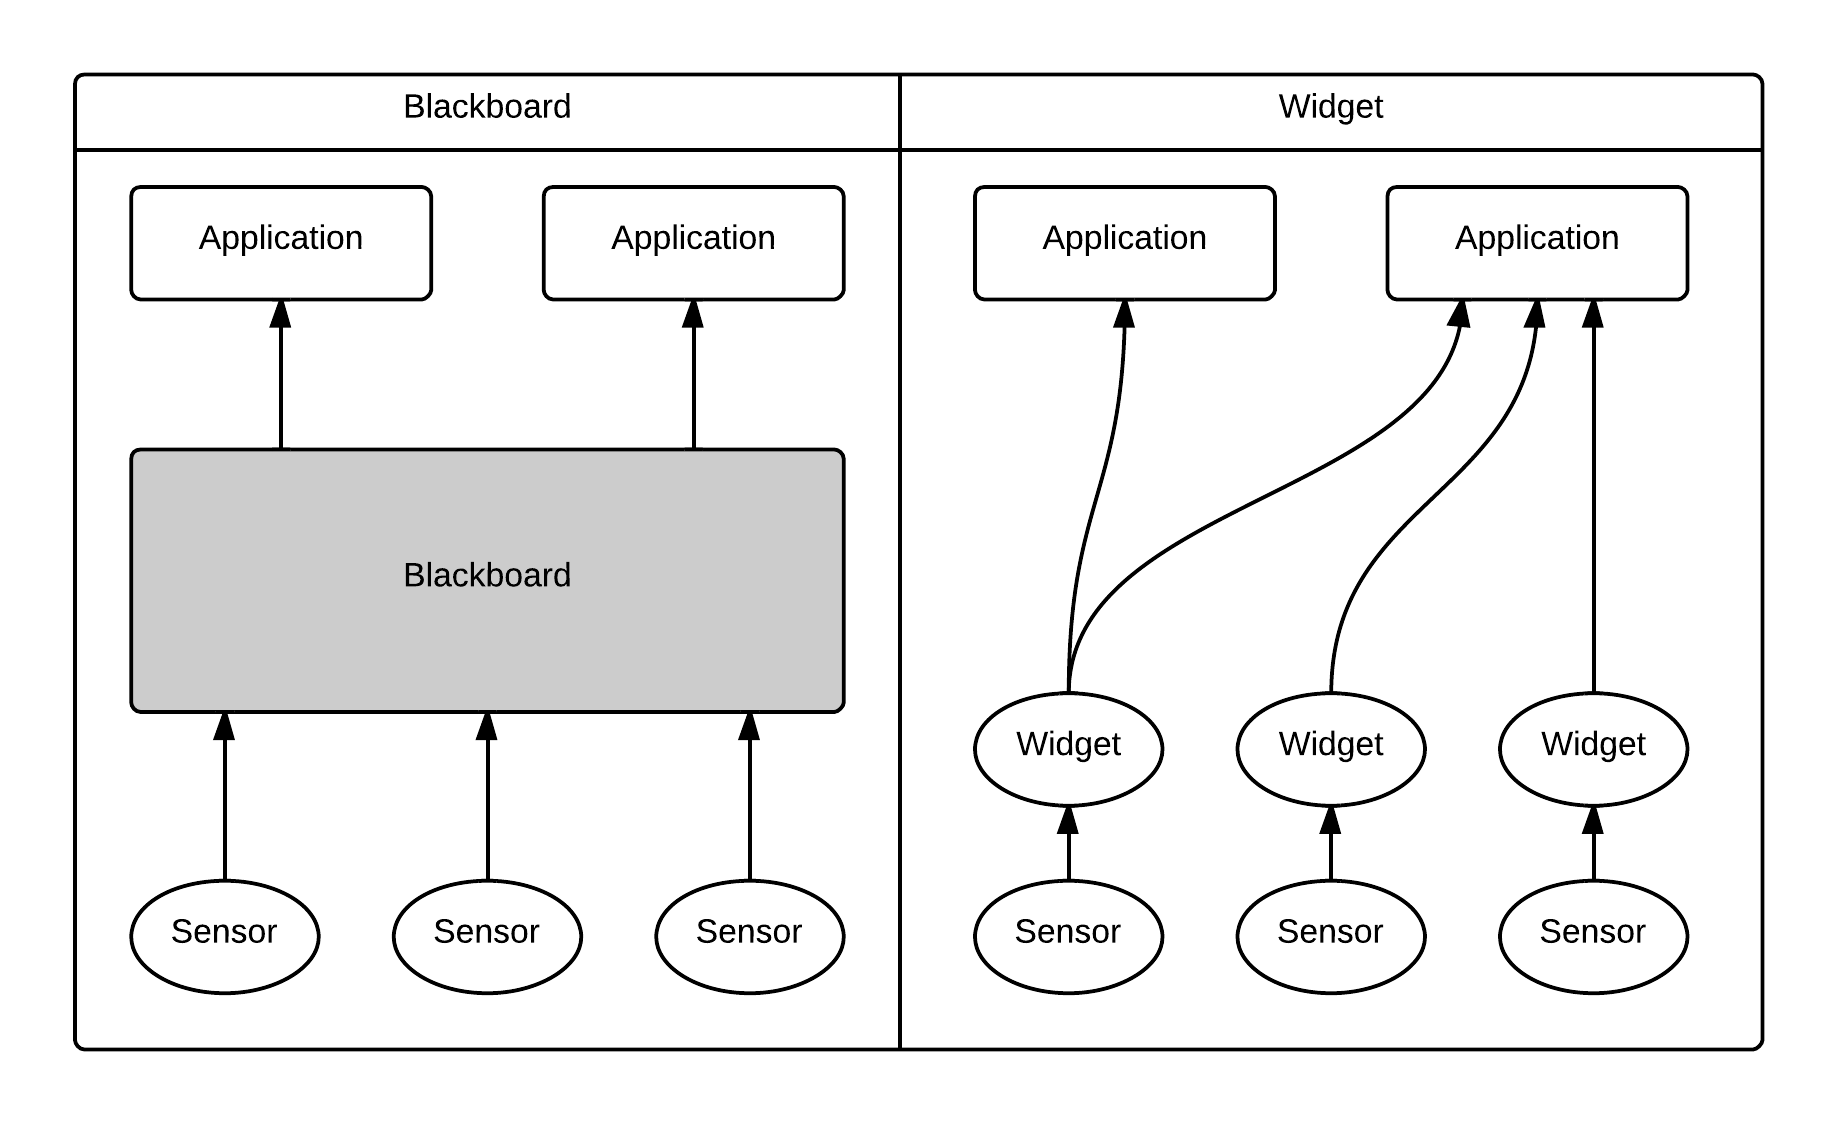
\includegraphics[width=\linewidth]{blackboard-widget.png}
\caption{Blackboard and widget-based approach}
\label{fig:blackboard-widget}
\end{figure}

The widget approach is an object-oriented distributed solution. Sensors encapsulated by widgets are available for application subscription. The solution is event based and applications are notified whenever a change to the sensor is occurring. This solution is object-oriented as the context is modeled with objects sent from sensor to application. This time and spare coupled solution stands in contrast to the blackboard approach which is a database and is therefore time- and spare uncoupled.

The solution differs a lot in the way the model context, but the main differers is in the way of delivering context from sensor to application. The solutions stands in great contrast when looking at space and time coupling. To briefly describe the theory, space coupling is weather or not the sender knows who the receiver of a message is. Time coupling is if the given message is only available in real-time. 

Where the blackboard at any time offers applications to go though it's context database, it does not offer notifying the application, as the blackboard is space uncoupled, and does not know about the application. The widget solution offers live updated only when they happens and only to the applications subscribing for the update.

Both solutions are very useful in different applications.

\todo Should the two examples stay?\\
For example a hospital system where you want to use the context framework to track patients, the blackboard solution seams to meet requirements best as you can, when needed, look up a patients whereabout in the hospital.

For a home automation system using sensors, sensor input is only interesting the moment it happens, and only to actuator whom it concern. When a person enters the room the light should go on instantly, only in the room where the person entered and only at the given time. 


\chapter{Design}
This chapter describes the different design choices we have though about in developing the framework.

To establish a vocabulary:
	Situation - A physical situation eg. A person sitting down

	Context - Context is knowing the situation and being able to react and be accordingly

	Context information - Every information that aggregates a context

\section{Grand Architecture}
When looking at the blackboard and widget based methods, we have decided that we want to include a little of both.

We want to do a centralized system where clients can register a predicate. A predicate could be that the client would like to be notified whenever the situation is that a person is sitting down.

The framework should be event-based so when ever the state of a clients predicate changes, an event will be fired to notify the client.  

This combines the blackboards centralization with the widgets time and space coupling making it transparent for the developer which sensor is actually given the input, but also having the space and time coupling from the widget based method.

With this our framework will be an If-this-then-that solution where the client can use sensor input for control without the  client developers having to put much though into using and managing sensors  


\section{Central}
 

\section{Encapsulation of Context-information}
Object-oriented encapsulation of context can be done in a variety of ways.

We have been looking at two different methods. Using a composite pattern and modeling with properties.

Using a composite pattern enforced relations between entities, entities being locations, persons, things or other real world objects.

Lets say we want to model a location with some rooms with some persons with different items or actions. Using the composite modeling we can have a location object containing room objects containing person objects containing item objects. We'll then have a relationship between the objects compositing the context being that a group of students is in room 3A04 at ITU all having phones in their pockets and all sitting down. This is a fairly complex, but a very extensible and flexible way to model situation (See fig \ref{fig:composite}). The downside to this method is that you can easily have an overflow of entities, and that it can be very complex and computation heavy to check against a  predicate.

The other method we are considering is more simple. Having a set of entities that we wish to track, eg persons. All context information relating to a person will be properties to the object. So to use the previous example, a person entity would then have a location property, being ITU room 3A04, a phone property begin true and a sitting property being true. This model is more easy to make, but it limits the developer to know very precisely what information is needed and should be tracked. The previous model had the advantage of being very flexible allowing more complex relations and situations. 

Both methods have pros and cons being how dynamic they are, how easily they can be implemented, and what performance they will have and that will be the parameters we'll look at when implementing the framework 

\begin{figure}
\centering
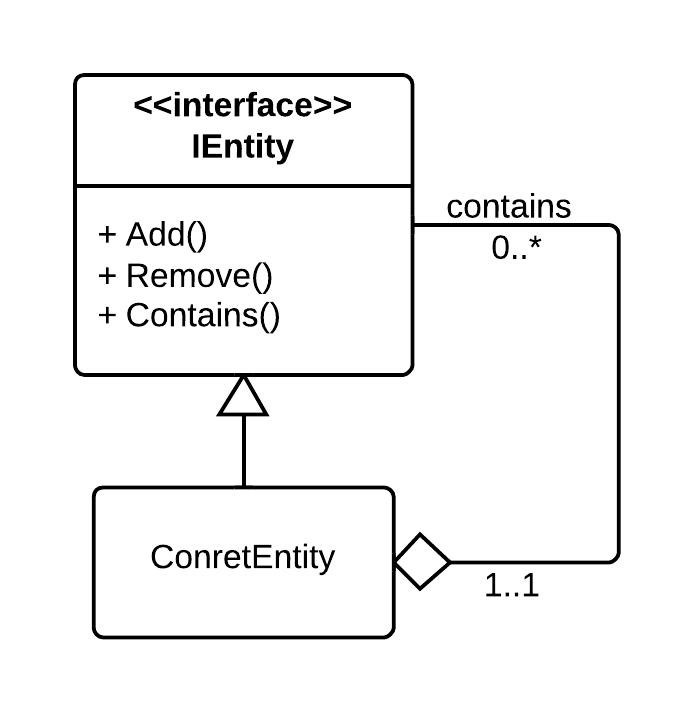
\includegraphics[width=200px]{composite.png}
\caption{Diagram illustrating composite modeling}
\label{fig:composite}
\end{figure}

\section{Widget}

\begin{figure}
\centering
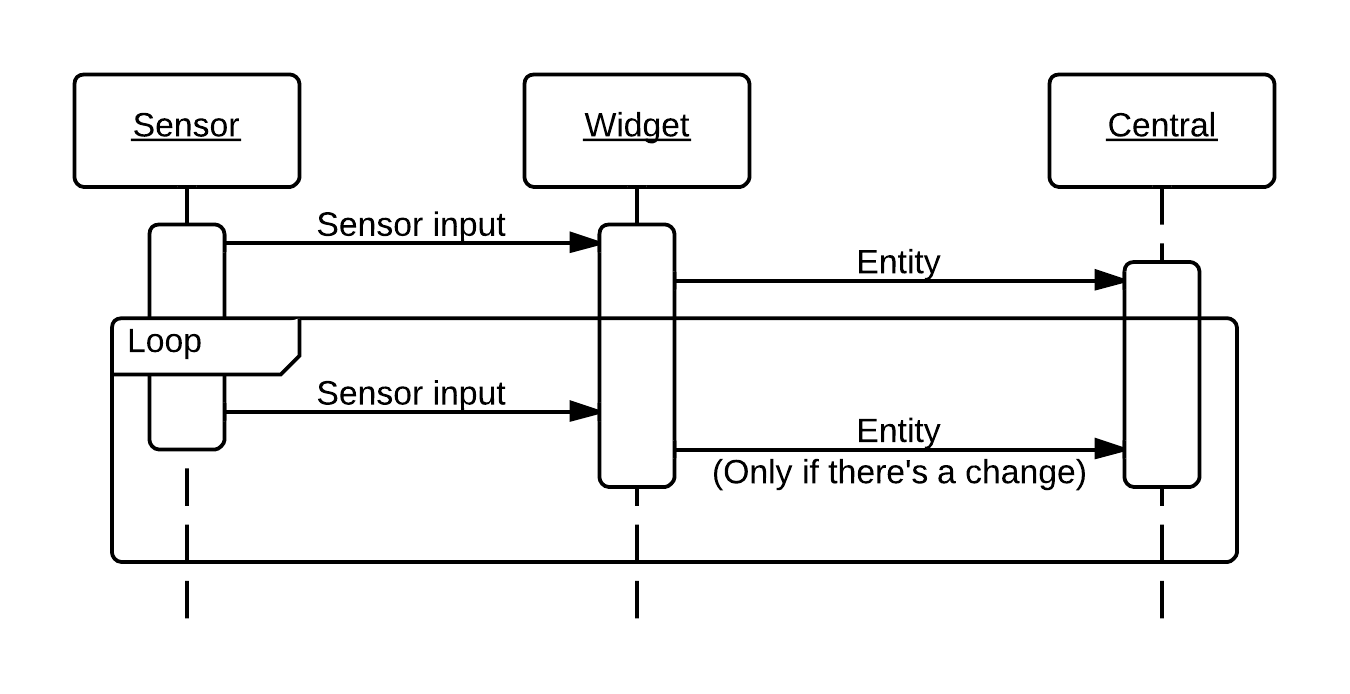
\includegraphics[width=\linewidth]{sequencediagram-widget.png}
\caption{Input flow from Widget to central}
\label{fig:seqwidget}
\end{figure}


In our framework widgets will translate sensor input to entities along with facilitating the communication to the central.

This approach have been chosen to make the system easily distributed as a small, maybe embedded, component can facilitate as widget translating the sensors input to entities before sending them to the central.

This approach will also reduce network load as the widget will only send updates to the central when changes occur. This stands in contrast to sending all sensor input to the central and making it process the data itself which could be useful in some cases.

Latests would also put more computational pressure on the central making it hard to scale to larger systems.


\section{Client}

The client will be the entry point into the framework facilitating the developers to subscribe to situations in the central and receive updates whenever an update to that situation occurred. 

\todo write more

\section{Dynamic Entity types}


\section{Communication}

Initially we decided that making the framework distributed would be out scoped, but as the project progressed it was decided to bring it into scope.

The reason for doing so is that our vision of having a centralized system distributing situation from sensors to clients is not very useful if not distributed.

For the framework two different communication protocols need to be implemented.\\

\begin{itemize}
	\item A protocol for establishing link between peers
	\item A protocol for send text/json messages for subscriptions, subscription events and, sensor events \\
\end{itemize}

We do not wish to bind our users to any concrete communication protocols. Therefore the communication will be interfaces so a concrete implementation can be dependency injected into the framework.

The framework will contain a default implementation build using the TCP/IP layer. For serialization we have chosen to use json. These decisions have been made so that developers are not bound to the .NET platform and can make clients and widgets in other languages like Java, or C directly on a micro controllers like Arduino.

For peer discovery we have chosen to use IP multicast. The central will broadcast itself for peers to discover. The peer, clients and widgets, will be listening on the multicast endpoint and will invoke an event when a central is discovered. See figure \ref{fig:widgetComHelper} and \ref{fig:clientComHelper} for a detailed view of the communication between client and central and widget and central

\begin{figure}
\centering
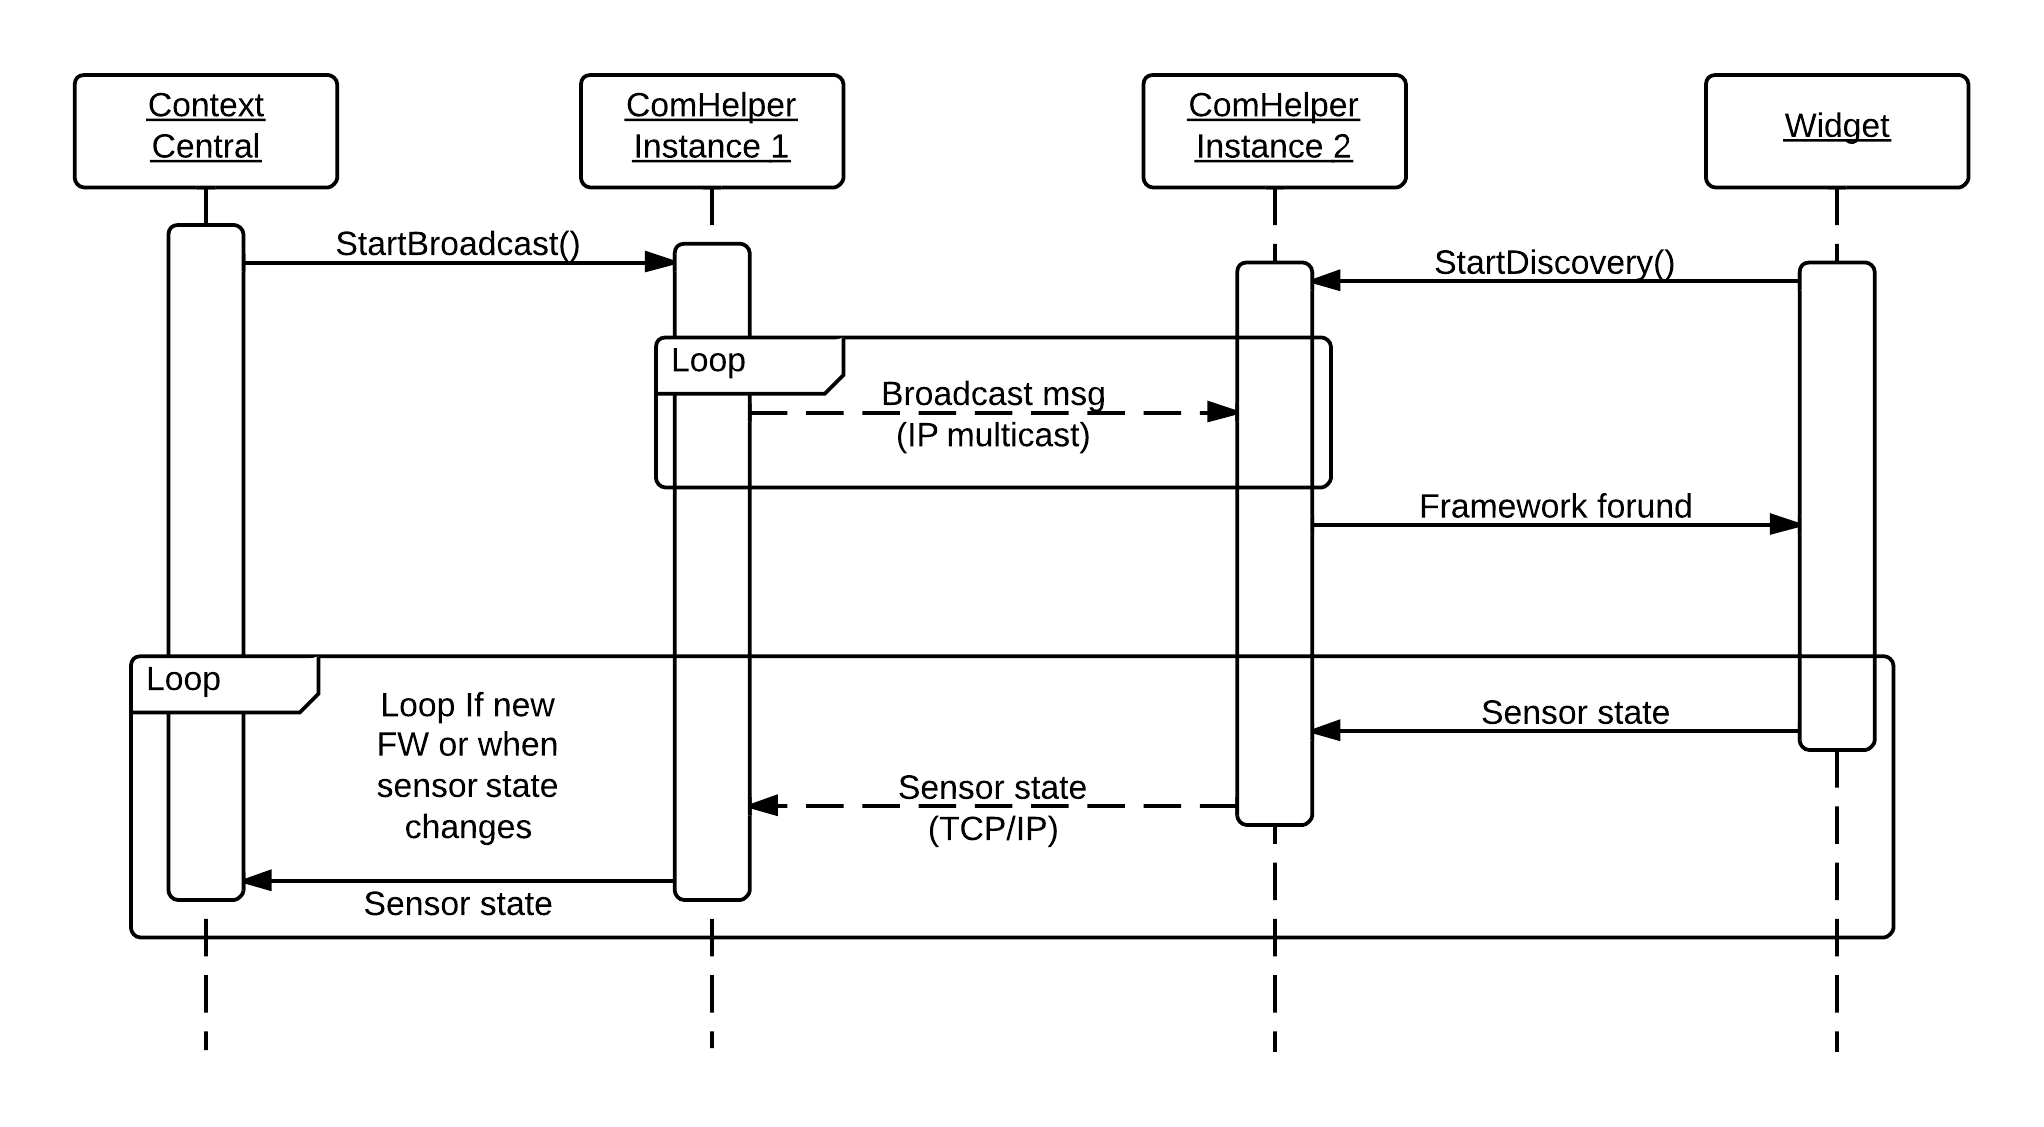
\includegraphics[width=\linewidth]{comHelperSequence-widget.png}
\caption{Widget to Central sequence diagram}
\label{fig:widgetComHelper}
\end{figure}

\begin{figure}
\centering
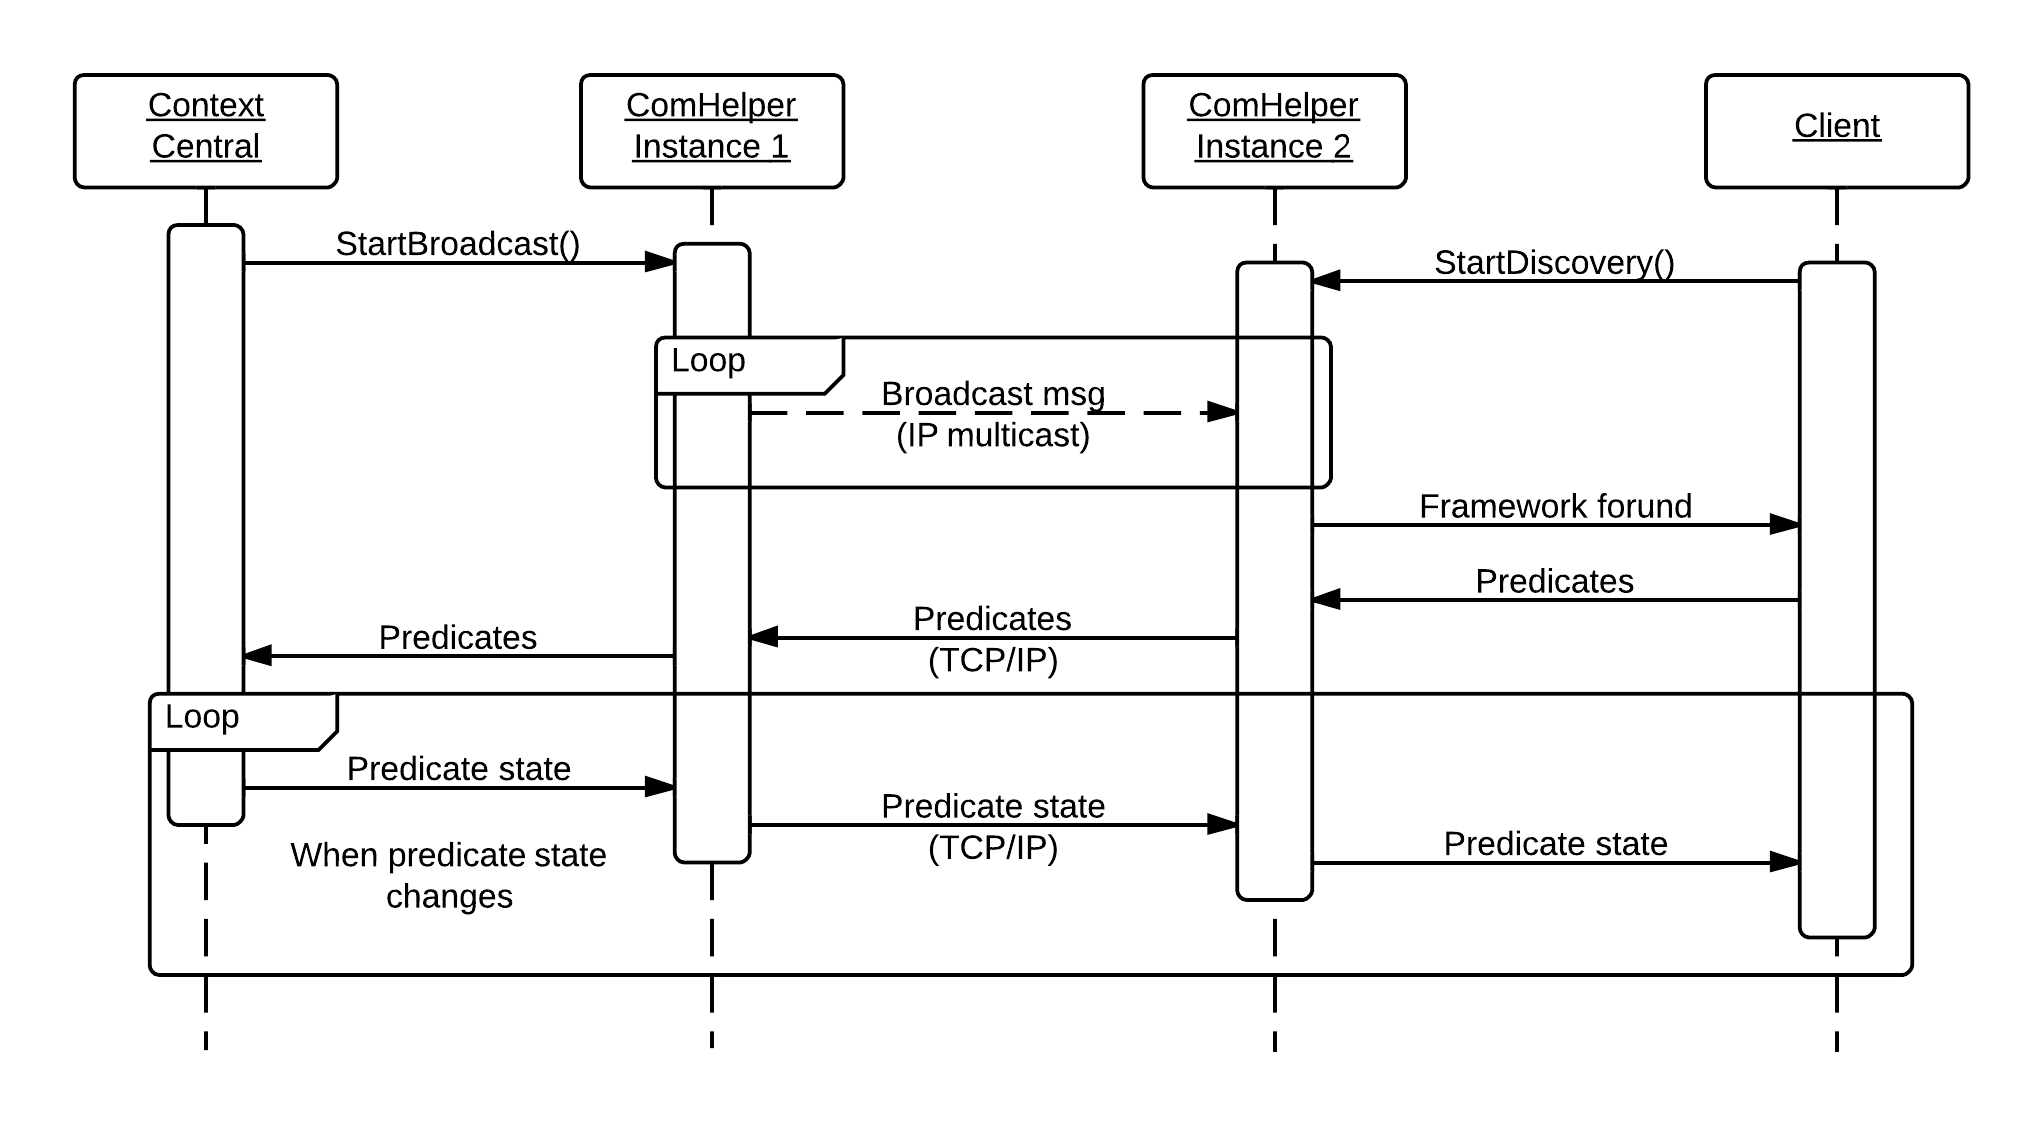
\includegraphics[width=\linewidth]{comHelperSequence-client.png}
\caption{Client to Central sequence diagram}
\label{fig:clientComHelper}
\end{figure}

\chapter{Implementation}


\section{Overview}

\begin{center}
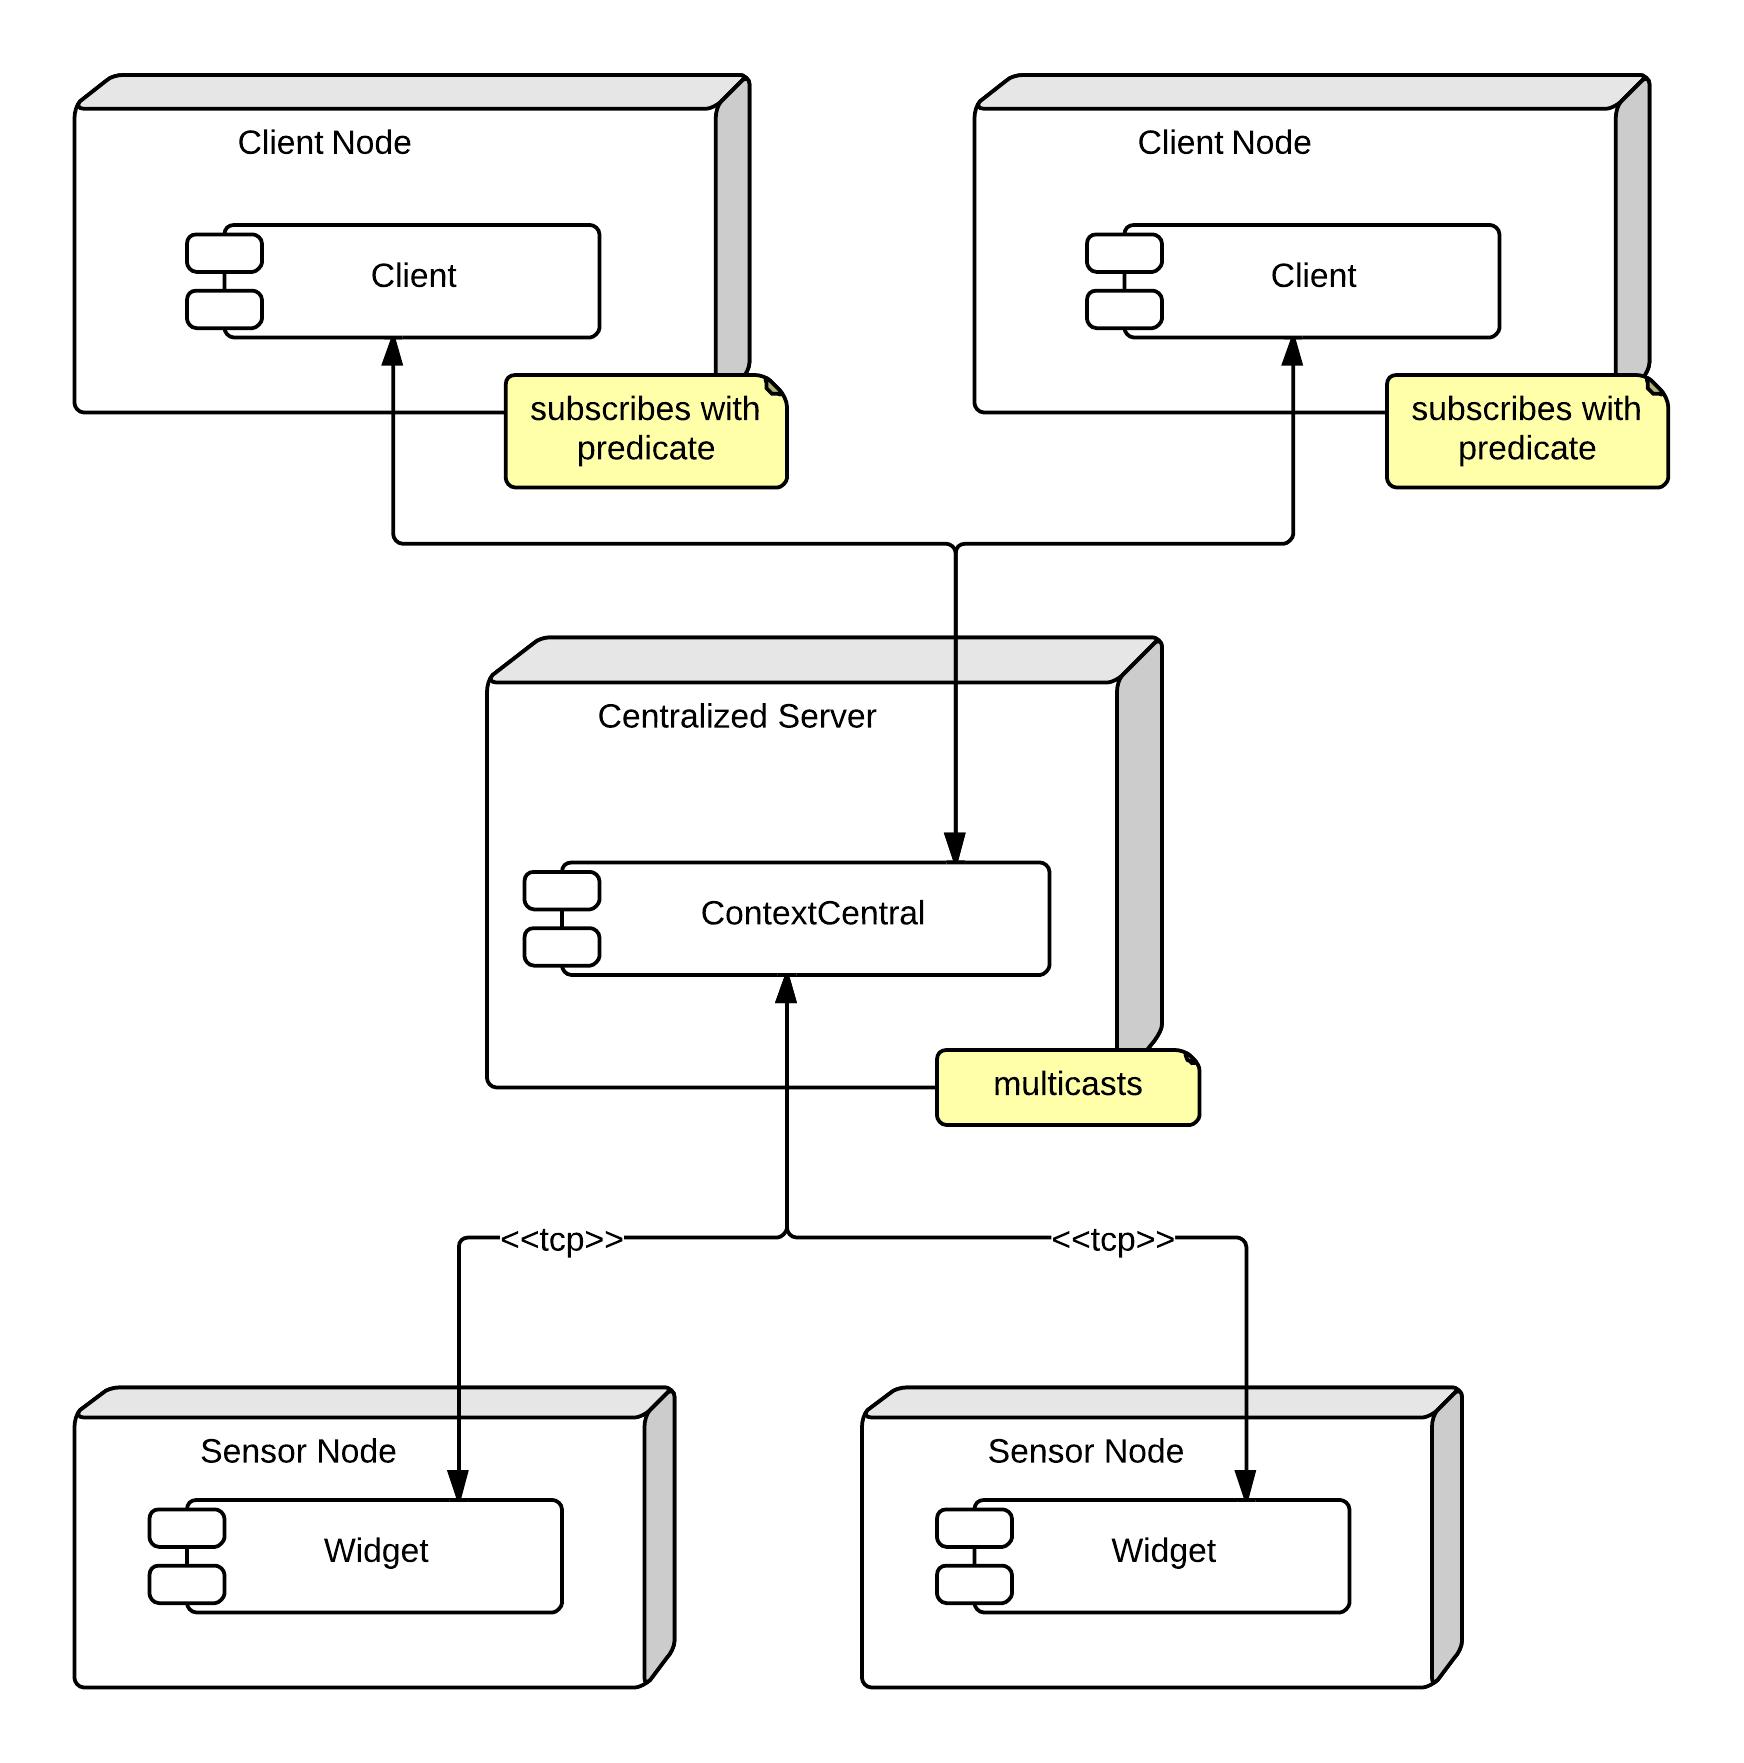
\includegraphics[scale=0.2]{ComponentDiagram.png}
\end{center}


\paragraph{The Client} is an observer interested in sensor data. It subscribes to a situation on the ContextCentral.

\paragraph{The Widget} wraps a sensor and translates the raw data to entities which are sent to the ContextCentral.

\paragraph{The ContextCentral} is the central for entity information and situations. When an entity is received from a widget, all stored situations are checked and subscribers notified accordingly.



\section{Encapsulation of Context}
Design choices in encapsulating context

Entities are generalized by the type IEntity, specifying general information for all entities.


\begin{center}
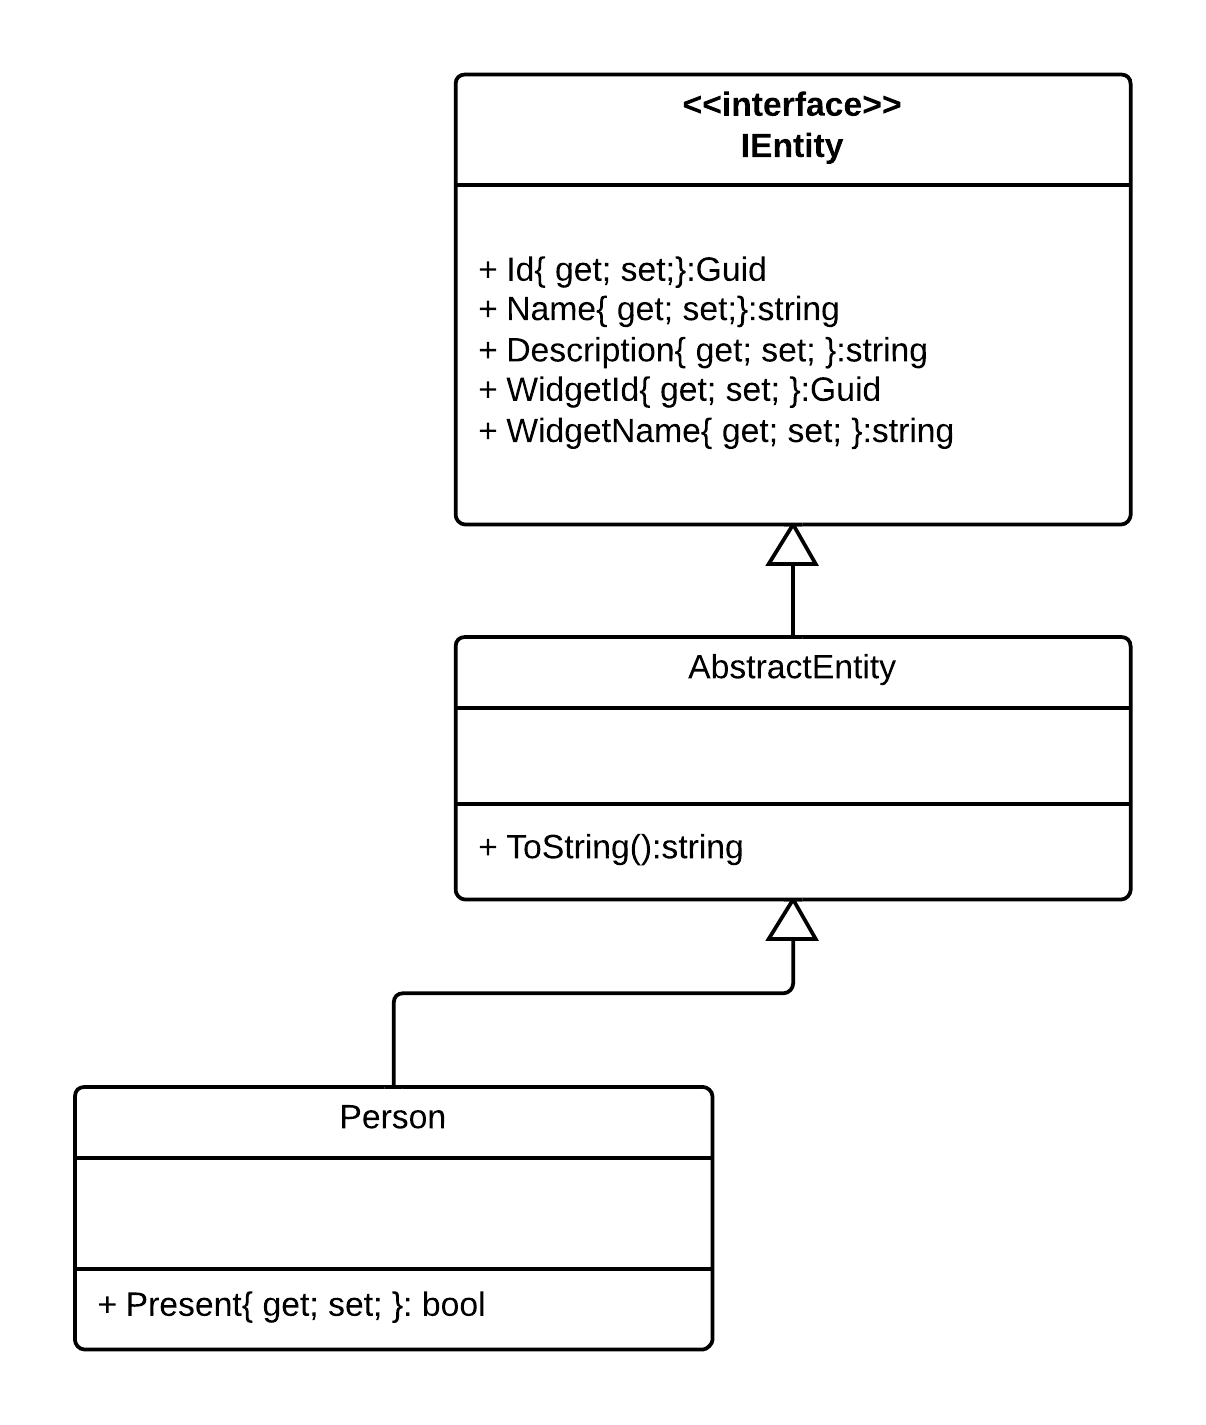
\includegraphics[scale=0.15]{ContextClassDiagram.png}
\end{center}


\section{Widget}

\section{Central}

\section{Client}

\section{Communication}



\chapter{Proof of concept}

\blockquote{
We can only evaluate the user experience afforded by the toolkit and its features by building applications that use it, and then evaluating them. While the toolkit itself can be evaluated on its technical criteria, the aspects of it that are designed to support a particular user experience can only be evaluated in the context of use and thus must be evaluated indirectly - through applications built with the toolkit. \cite{Infrastructure (2003)} \\}

In previous chapters we evaluated the framework on it's technical criteria by the design and choices made. In this chapter we will answer to our \textit{Goal 2} by implementing the framework.

\section{Motivation}

%Scrum is a popular agile process of developing software. Originally thought as using a whiteboard for scheduling development tasks, it has been hard for to make use of Scrum in distributed teams, or 



Scrum is a popular agile process for developing software. Center of focus is the whiteboard where tasks are coordinated, estimated and assigned. For more on Scrum see \textit{scrum.org}.

We ourselves have used Scrum for several projects but never with the pleasure of a physical Scrumboard. We never had a room allocated and it simply wasn't possible to maintain a physical Scrumboard in a new space every day. A lot of tools for this problem have sprung up\footnote{Confluence, Scrumwise, Team Foundation, Trello} and made Scrum possible in this scenario, and even for a fully distributed team who would not be gathered physically in the first place.

While we have never used a whitebord for a full Scrum project, we have used it occasionally for single work days. We believe the physical board is important for:

\begin{itemize}
\item Always being able to turn ones head to the huge todo list is great motivation
\item No need for projecting a software tool during Scrum meetings
\end{itemize}


We have established our opinion that the presence of the whiteboard is important. The software tools for Scrum are confined to individuals computers and are not central like the whiteboard, which is why they lack this presence.

If you are able to maintain a physical Scrumboard, another problem surfaces. There is one great point where the whiteboard is lacking; It's Analog. Maintaining the data is all manual translation form the board to a spreadsheet or the likes.

%\begin{itemize}
%\item[] \Large{There is no solution today that digitalizes the whiteboard while maintaining it's presence}
%\end{itemize}

%\normalsize
%\vspace{0.2cm}

While this project does not cover implementing a Scrumboard which would solve these problems, we have still chosen this as proof of concept because we think it's an interesting topic.


\section{Context awareness}

There are two situations we deem important which we want the Scrumboard to act upon:

\begin{itemize}
\item The standup meeting: When more than one person is standing in front of the Board
\item An individual closeup with the board
\end{itemize}

Actuation on these situations is purely graphical. There will be change in the graphical interface according to which information the interactors are interested in given the situation.

\begin{itemize}
\item Standup
\item Closeup
\item Overview. This view is our default for when none of the other contexts are true
\end{itemize}


\todo{more explanation of the context involved and how we'll represent it with the framework...}



\section{Implementation}

The Context-aware Scrumboard consists of three parts: The Widget, The Central and the Scrumboard. These parts are in our case distributed and communicate by the TcpHelper implemented for the framework.


\paragraph{The Widget} blah\\

\begin{figure}[B]
\begin{lstlisting}
//Choose a logging instance if any
var log = Console.Out;

//Instantiate a network helper. Here passing the logging target
//alternatively instantiate as new TcpHelper(); if no logging is needed
var comHelper = new OconTcpCom(log);

//Instantiate the client with communication, log, and params of situation names strings
var oconClient = new OconClient(comHelper, log, StandupSituationString, CloseupSituationString);

//Subscribe a delegate to be run when a situation change event is fired
oconClient.SituationStateChangedEvent += (sender, args) => UpdatePicture(args.SituationName, args.State);
\end{lstlisting}
\caption{Client usage from OconScrumBoard.MainViewModel}
\label{code:OconWidget}
\end{figure}


\paragraph{The Central} hauwd

\begin{figure}[H]
\begin{lstlisting}
//Choose a logging instance if any
var log = Console.Out;

//Instantiate a network helper. Here passing the logging target
//alternatively instantiate as new TcpHelper(); if no logging is needed
var comHelper = new OconTcpCom(log);

//Instantiate the client with communication, log, and params of situation names strings
var oconClient = new OconClient(comHelper, log, StandupSituationString, CloseupSituationString);

//Subscribe a delegate to be run when a situation change event is fired
oconClient.SituationStateChangedEvent += (sender, args) => UpdatePicture(args.SituationName, args.State);
\end{lstlisting}
\caption{Client usage from OconScrumBoard.MainViewModel}
\label{code:OconCentral}
\end{figure}

\paragraph{The Scrumboard} blah \\

\begin{figure}[H]
\begin{lstlisting}
//Choose a logging instance if any
var log = Console.Out;

//Instantiate a network helper. Here passing the logging target
//alternatively instantiate as new TcpHelper(); if no logging is needed
var comHelper = new OconTcpCom(log);

//Instantiate the client with communication, log, and params of situation names strings
var oconClient = new OconClient(comHelper, log, StandupSituationString, CloseupSituationString);

//Subscribe a delegate to be run when a situation change event is fired
oconClient.SituationStateChangedEvent += (sender, args) => UpdatePicture(args.SituationName, args.State);
\end{lstlisting}
\caption{Client usage from OconScrumBoard.MainViewModel}
\label{code:OconClient}
\end{figure}


\todo{This solution with the elements from blackboard makes development very uncoupled. The bloackboard requires a concensus and so Widget/sensor and client can be implemented independently}

\chapter{Conclusion}

\begin{thebibliography}{9}

\bibitem{Dey and Abowd (2000)}
  Dey, A. K., and Abowd, G.D.
  \emph{Towards a better understanding of context and context-awareness. Workshop on the What, Who, Where, When and How Context-awareness, afflicted with the 2000 ACM Conference on Human Factors in Computer Systems},
  2000.
  
\bibitem{Dey and Newberger (2009)}
  	Anind K. Dey and Alan Newberger
  	\emph{Support for Context-Aware Intelligibility and Control}, 2009
  
  
\bibitem{Infrastructure (2003)}
  W. Keith Edwards, Victoria Bellotti, Anind K. Dey,
  Mark W. Newman.
  \emph{Stuck in the Middle: The Challenges of
  User-Centered Design and Evaluation for Infrastructure},
  2003.
  
\bibitem{Context-aware computing (2010)}
	Anind K. Dey
	\emph{Context-aware computing} in Ubiquitous Computing Fundamentals, 2010, 321-352

\end{thebibliography}
\chapter{Appendixes}

\end{document}
